% \problemname{Mineral deposits}
\problemname{Złoża mineralne}

\illustration{.3}{img/turnbull.jpg}{Eroding mud face exposing new minerals. Photo: Michael D.\ Turnbull, licence: CC BY-SA.}

\noindent
% You handle signal processing for an extra-terrestrial mining company, and your vessel is currently approaching an asteroid. 
Zajmujesz się przetwarzaniem sygnałów dla pozaziemskiej firmy wydobywczej, a twój statek właśnie zbliża się do asteroidy. 
% Preliminary scans show the presence of $k$~mineral deposits on the asteroid, but their precise locations are unknown.
Wstępne skany wskazują na obecność $k$~złóż minerałów na asteroidzie, ale ich dokładne lokalizacje nie są znane.

\medskip

% The surface of the asteroid can be seen as a grid of integer coordinates.
Powierzchnia asteroidy może być postrzegana jako siatka współrzędnych całkowitych.
% Each of the mineral deposits is located at unknown integer coordinates such that the $i$th deposit has coordinates $(x_i, y_i)$ with  
Każde ze złóż mineralnych znajduje się w nieznanych współrzędnych całkowitych, tak że $i$-te złoże ma współrzędne $(x_i, y_i)$ spełniające
% $-b \le x_i \le b$ and $-b\le y_i \le b$ %constraint:depositcoords
$-b \le x_i \le b$ oraz $-b\le y_i \le b$ %constraint:depositcoords
% for some integer $b$ corresponding to the size of your initial scan.
dla pewnej liczby całkowitej $b$ odpowiadającej rozmiarowi twojego początkowego skanu.

% To determine the precise locations of the mineral deposits, you may send probes to the surface of the asteroid. 
Aby określić dokładne położenie złóż minerałów, możesz wysłać na powierzchnię asteroidy sondy. 
% The probes are sent out in waves of several probes at once.
Sondy są wysyłane w porcjach po kilka sond jednocześnie.

% Say you sent a wave of $d$~probes to the surface at coordinates $(s_j,t_j)$ for $1\leq j\leq d$.
Powiedzmy, że wysłałeś jedną porcję $d$~sond na powierzchnię na współrzędne $(s_j,t_j)$ dla $1\leq j\leq d$.
% When a probe arrives at its coordinates, it determines the Manhattan distances to each of the $k$~mineral deposits and sends the distances back to the ship. 
Kiedy sonda dociera do swoich współrzędnych, określa odległości w metryce Manhattan do każdego z $k$~złóż minerałów i wysyła odległości z powrotem na statek. 
% All data packets arrive at the same time, and it is not possible to determine which probes returned which distances. 
Wszystkie pakiety danych docierają w tym samym czasie i nie jest możliwe określenie, które sondy zwróciły jakie odległości. 
% Thus the wave returns the $k\cdot d$ integer distances
Tak więc porcja zwraca $k\cdot d$ odległości całkowitych
% \[|x_i-s_j| + |y_i - t_j| \qquad\text{for all } i \in \{1,\ldots,k\} \text{ and } j \in\{ 1,\ldots,d\}\,.\]
\[|x_i-s_j| + |y_i - t_j| \qquad\text{dla każdego } i \in \{1,\ldots,k\} \text{ oraz } j \in\{ 1,\ldots,d\}\,.\]

% You need to minimise the number of waves of probes that is sent to the surface.
Musisz zminimalizować liczbę porcji sond, które są wysyłane na powierzchnię.


\section*{Interakcja}

% This is an interactive problem.
Jest to problem interaktywny.
% Interaction begins with you reading a single line containing three integers $b$, $k$, and $w$:
Interakcja rozpoczyna się od przeczytania pojedynczego wiersza zawierającego trzy liczby całkowite $b$, $k$ oraz $w$:
% the grid's boundary~$b$,
granica siatki~$b$,
% the number~$k$ of mineral deposits,
liczbę złóż minerałów~$k$,
% and the maximum number~$w$ of waves you may send.
i maksymalna liczba~$w$ porcji, które możesz wysłać.

% You then ask at most $w$ queries, each corresponding to a wave.
Następnie zadajesz co najwyżej $w$ zapytań, każde odpowiadające jakiejś porcji.
% A query consists of \texttt{?} followed by $2d$ integers separated by space, such as ``\texttt{?} $s_1$ $t_1$ $\cdots$ $s_d$ $t_d$'', where the number~$d$ of probes in this wave must satisfy
Zapytanie składa się z \texttt{?}, po którym następuje $2d$ liczb całkowitych oddzielonych spacją, na przykład ``\texttt{?} $s_1$ $t_1$ $\cdots$ $s_d$ $t_d$'', gdzie liczba~$d$ sond w tej porcji musi spełniać wymagania
$1\leq d\leq 2000$. % constraint:wavesize
% The values $(s_i,t_i)$ are interpreted as the coordinates of the $i$th probe and must satisfy
Wartości $(s_i,t_i)$ są interpretowane jako współrzędne $i$-tej sondy i muszą spełniać
% $-10^8 \leq s_i \leq 10^8$ and $-10^8 \leq t_i \leq 10^8$. % constraint:probecoordinates
$-10^8 \leq s_i \leq 10^8$ oraz $-10^8 \leq t_i \leq 10^8$. % constraint:probecoordinates
% The response is a single line with $k \cdot d$ integers in non-decreasing order: all pairs of Manhattan distances between the mineral deposits and the probe coordinates.
Odpowiedzią jest jeden wiersz zawierający $k \cdot d$ liczb całkowitych w kolejności niemalejącej: wszystkie pary odległości w metryce Manhattan pomiędzy złożami mineralnymi oraz współrzędnymi sondy.
% The total number of probes across all waves may not exceed
Całkowita liczba sond we wszystkich porcjach nie może przekroczyć
$2\cdot 10^4.$ % constraint:totalprobes

% Interaction ends with you printing a single line consisting of \texttt{!} followed by $k$ points $x_1, y_1, x_2, y_2, \ldots x_k, y_k$, separated by space.
Interakcja kończy się wypisaniem pojedynczego wiersza składającego się ze znaku \texttt{!}, po którym następuje $k$ punktów $x_1, y_1, x_2, y_2, \ldots x_k, y_k$, oddzielone spacją.
% This must be your last line of output.
To musi być twój ostatni wiersz wyjścia.

% Your submission is considered correct if you print all locations of the mineral deposits.
Twoje zgłoszenie zostanie uznane za poprawne, jeśli wypiszesz wszystkie lokalizacje złóż minerałów.
% You may print them in any order.
Możesz je wypisać w dowolnej kolejności.

\section*{Ograniczenia i punktacja}

% We always have 
Zawsze jest spełnione 
$1\leq b \leq 10^8$, % constraint:b
$1 \leq k \leq 20$, % constraint:k
% and
oraz
$2 \le w \le 10^4$. % constraint:w

% Your solution will be tested on a set of test groups, each worth a number of points.
Twoje rozwiązanie zostanie przetestowane na zestawie grup testowych, z których każda jest warta pewną liczbę punktów.
% Each test group contains a set of test cases.
Każda grupa testowa zawiera zestaw przypadków testowych.
% To get the points for a test group you need to solve all test cases in the test group.
Aby uzyskać punkty za daną grupę testową należy rozwiązać wszystkie przypadki testowe w tej grupie.
% Your final score will be the maximum score of a single submission.
Twój ostateczny wynik będzie maksymalnym wynikiem pojedynczego zgłoszenia.

\medskip
\begin{tabular}{lll}
% Group & Points & Constraints \\\hline
Grupa & Punkty & Ograniczenia \\\hline
  $1$ & $9$ & $k = 1, w = 10^4$\\
  $2$ & $19$ & $w \ge 500$\\
  $3$ & $11$ & $w \ge 210$\\
  $4$ & $7$ & $w \ge 130$\\
%   $5$ & $20$ & $w \ge 3$, $b \le 10^4$\\
  $5$ & $20$ & $w \ge 3$, $b \le 10^4$\\
%   $6$ & $15$ & $w \ge 3$, $b \le 10^7$\\
  $6$ & $15$ & $w \ge 3$, $b \le 10^7$\\
%   $7$ & $19$ & \emph{No further constraints}
  $7$ & $19$ & \emph{Brak dalszych ograniczeń}
\end{tabular}

\section*{Przykład}

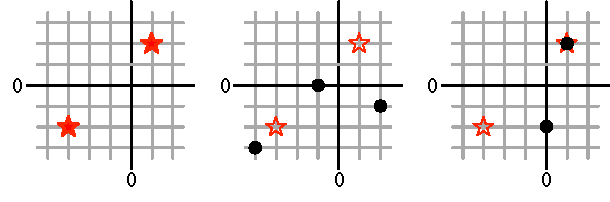
\includegraphics[width=.6\textwidth]{img/sample1.pdf}

% In this example, there are $k=2$ mineral deposits at positions $(1,2)$ and $(-3,-2)$, shown as red stars.
W tym przykładzie, na pozycjach $(1,2)$ oraz $(-3,-2)$ znajdują się $k=2$ złoża mineralne, zareprezentowane jako czerwone gwiazdy.
% In the first wave, you might send $d=3$ probes to $(-4,-3)$, $(-1, 0)$, and $(2,-1)$, shown as black dots.
W pierwszym rzucie możesz wysłać $d=3$ sondy na pozycje $(-4,-3)$, $(-1, 0)$ oraz $(2,-1)$, zareprezentowane jako czarne kropki.
% This wave would return the $6$ distances \[
Ta porcja zwróciłaby $6$ odległości \[
  2, 4, 4, 4, 6, 10\,.
\]
% In the next wave, you might send $d=2$ probes to $(1,2)$ and $(0,-2)$.
 W następnej porcji można wysłać sondy $d=2$ do $(1,2)$ oraz $(0,-2)$.
% This wave would return the $4$ distances \[
Ta porcja zwróciłaby $4$ odległości \[
  0, 3, 5, 8\,.
\]
